\begin{figure}
	\centering
	
    \begin{minipage}{0.5\linewidth}
    		\subfigure[][PnlP]{\label{fig:pnlp}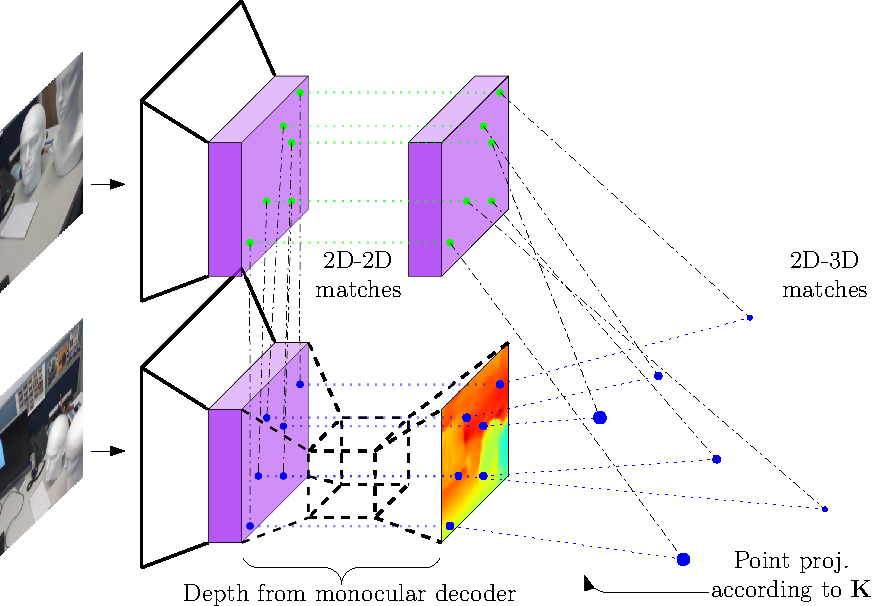
\includegraphics[width=0.9\linewidth]{method/pnlp}}
    \end{minipage}\hfill
	\begin{minipage}{0.5\linewidth}
   		\subfigure[][IClP]{\label{fig:iclp}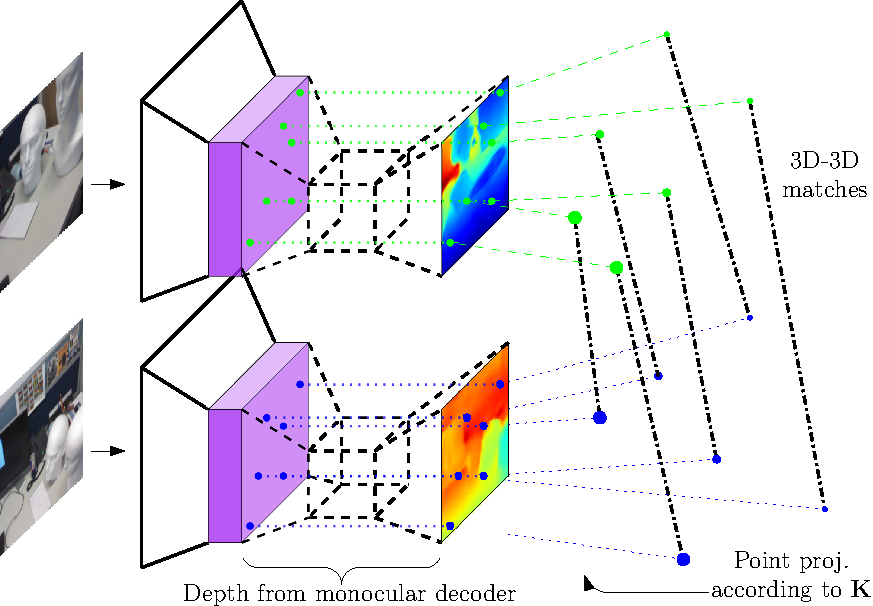
\includegraphics[width=0.9\linewidth]{method/iclp}}
	\end{minipage}
	
	\caption[Relative pose computation methods]{\textbf{Our two method for relative pose computation:} \ref{fig:pnlp} we compute the relative 6-\ac{dof} from 2D-3D correspondances using a \ac{pnp} like method. \ref{fig:iclp} we manage to align two point clouds projected from learned depth maps to recover the realtive pose of the two images, using an \ac{icp} like algorithm.\label{fig:relative_pose}}
\end{figure}
